
%--- Outline ---
\begin{frame}{Outline}
  \begin{itemize}
    \item What is Sementic Segmentation?
    \item How Can We Improve It? (Data Augmentation)
    \item Real-World Example: Disaster Images
    \item Project: Can AI-Generated Images Help?
  \end{itemize}
\end{frame}

\begin{refsection}
  \begin{frame}
    \centering
    \vspace{2.5cm}
    {\LARGE \textbf{Introduction to Sementic Segmentation}}
  \end{frame}
\end{refsection}

\begin{refsection}
  \begin{frame}{What is Semantic Segmentation?}
    \begin{itemize}
      \item Semantic segmentation means labeling each pixel in an image with a class (e.g., building, road, water).
      \item It helps computers understand exactly where objects are in a picture.
    \end{itemize}
    \begin{figure}
      \centering
      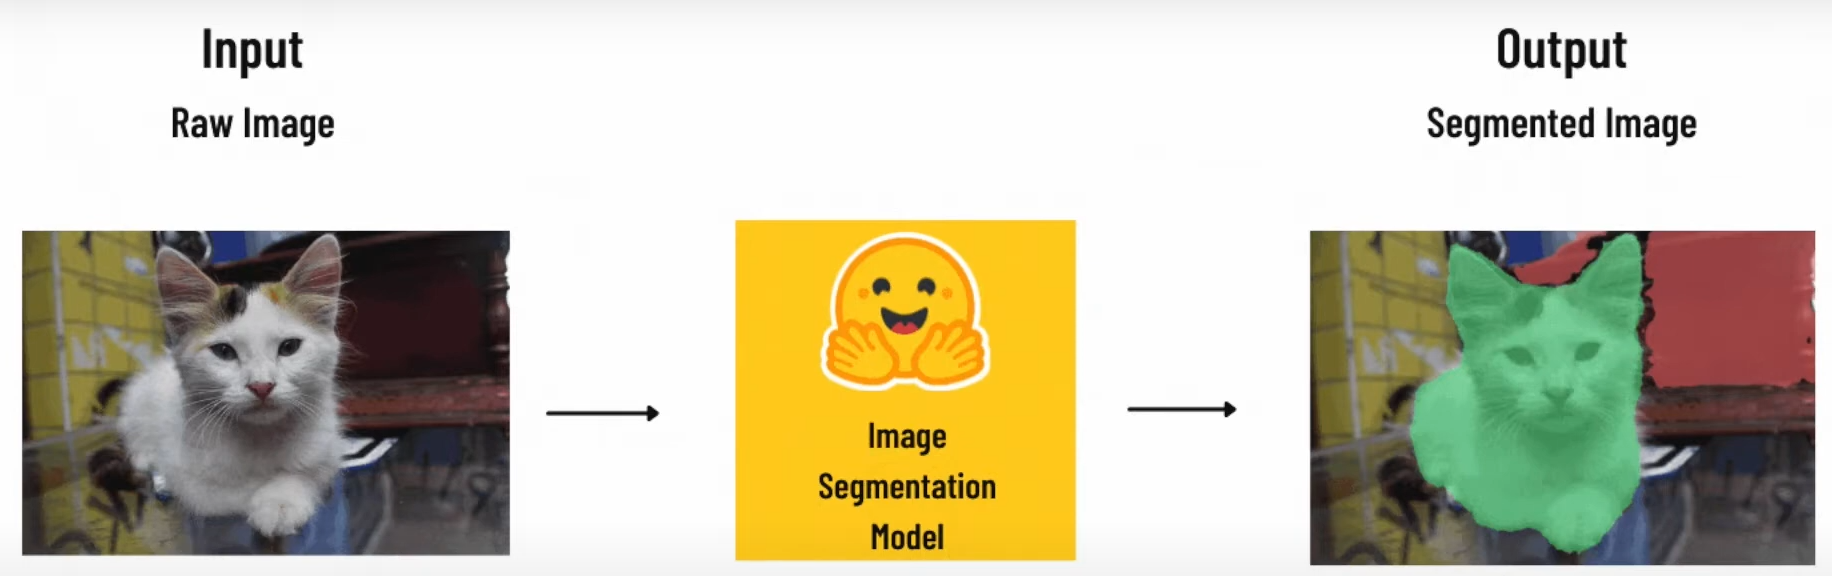
\includegraphics[width=1.0\linewidth]{image_ss.png}
      \caption[]{\scriptsize Illustration of Image Segmentation.}
    \end{figure}

  \end{frame}
\end{refsection}


\begin{refsection}
  \begin{frame}{SegEarth-OV: Training-Free Open-Vocabulary Segmentation}
    % \begin{itemize}
    %   \item \textbf{SegEarth-OV}~\parencite{liSegEarthOVTrainingFreeOpenVocabulary2025} is a recent method for open-vocabulary segmentation in remote sensing.
    %   \item It does not require extra training for new classes—just provide a text prompt!
    %   \item Enables flexible and efficient extraction of objects (e.g., buildings, roads, water) from satellite images.
    %   \item Useful for rapid response in disaster scenarios where new object types may appear.
    % \end{itemize}
    \begin{figure}
      \centering
      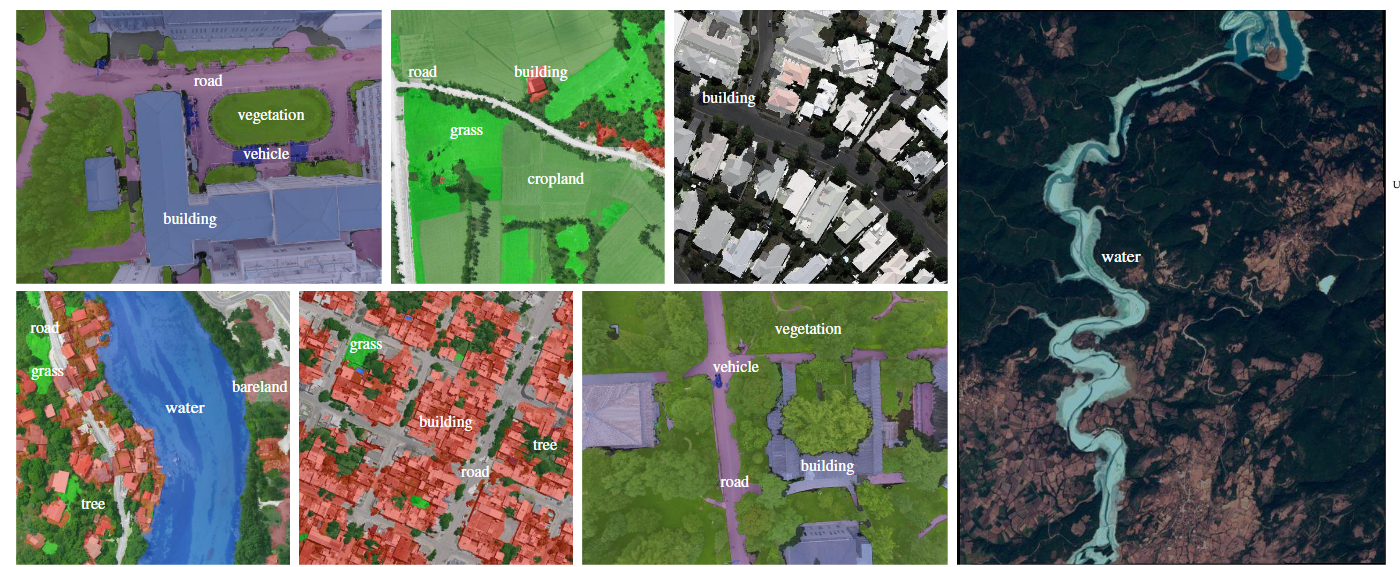
\includegraphics[width=0.95\linewidth]{segearthov.png}
      \caption[]{\scriptsize Visualization and performance of SegEarth-OV on open-vocabulary semantic segmentation of remote sensing images.~\parencite{liSegEarthOVTrainingFreeOpenVocabulary2025}.}
    \end{figure}
    \bottomleftrefs
  \end{frame}
\end{refsection}

% \begin{refsection}
%   \begin{frame}{Change Detection for Remote Sensing: Building Extraction}
%     % \begin{itemize}
%     %   \item Semantic segmentation is widely used in remote sensing to extract buildings from satellite images.
%     %   \item Specialized neural networks, such as Localization U-Net, can accurately locate and segment buildings.
%     % \end{itemize}
%     \begin{figure}
%       \centering
%       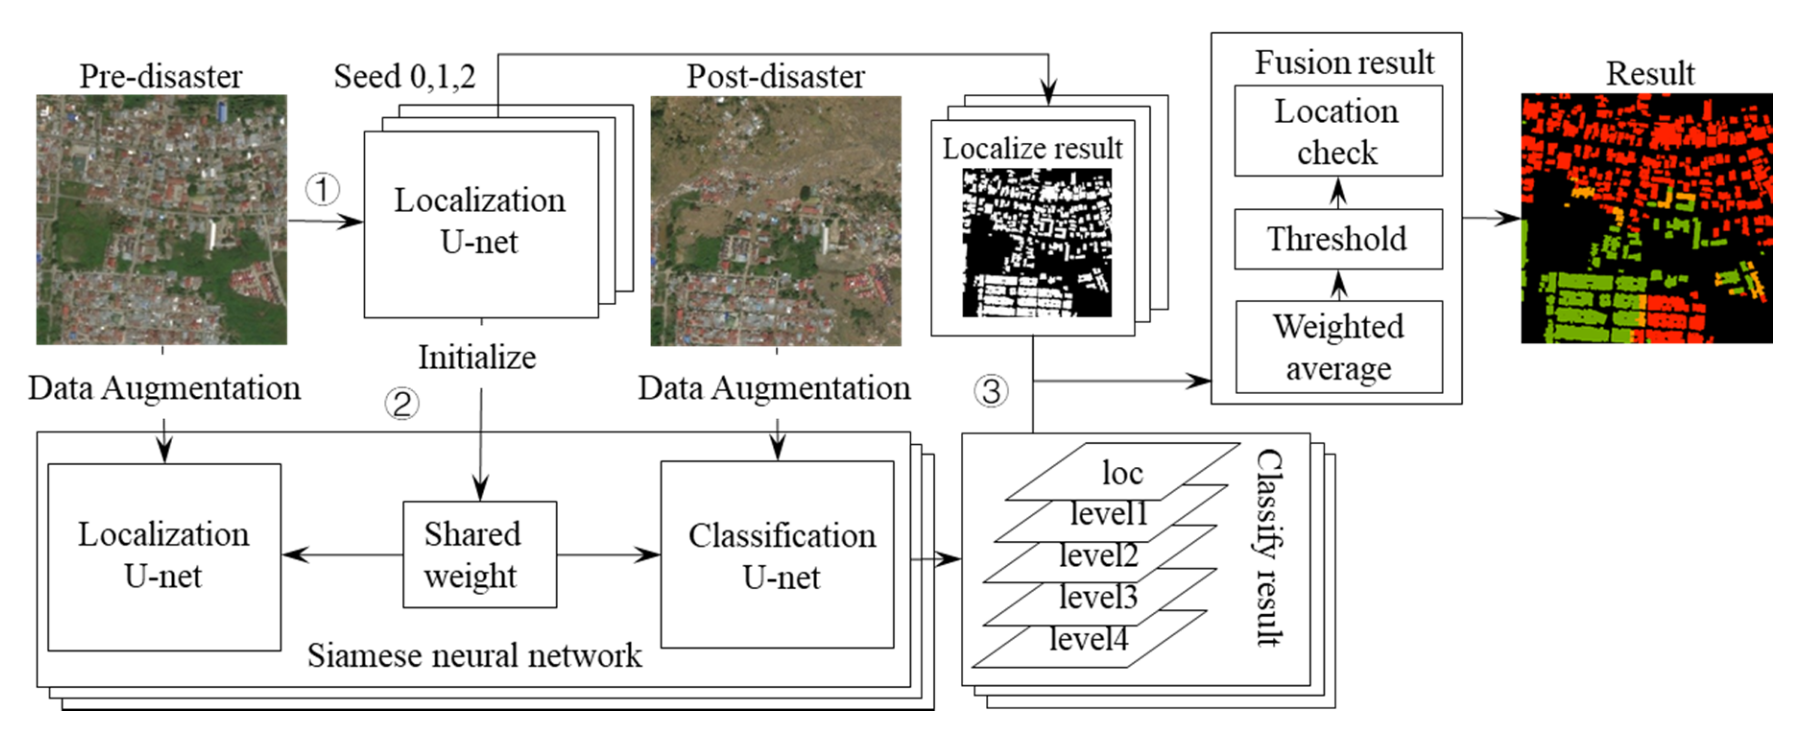
\includegraphics[width=1.0\linewidth]{chuyiwu_rs.png}
%       \caption[]{\scriptsize The overall framework. Localization U-Net is used to locate buildings.~\parencite{wuBuildingDamageDetection2021}}
%     \end{figure}
%     \bottomleftrefs
%   \end{frame}
% \end{refsection}


%--- Section: Data Augmentation ---
\begin{refsection}
  \begin{frame}
    \centering
    \vspace{2.5cm}
    {\LARGE \textbf{How Can We Improve Sementic segmentation?}\\[0.5em]
    \textbf{(Data Augmentation)}}
  \end{frame}
  \end{refsection}
  
  %--- Data Augmentation: Why? ---
  \begin{refsection}
  \begin{frame}{Why Use Data Augmentation?}
    \begin{minipage}{0.48\linewidth}
      \begin{itemize}
        \item Sometimes we do not have enough images to train a good model.
        \item Data augmentation means making new images from existing ones.
        \item It helps the model learn better and avoid mistakes.
      \end{itemize}
    \end{minipage}%
    \hfill
    \begin{minipage}{0.48\linewidth}
      \centering
      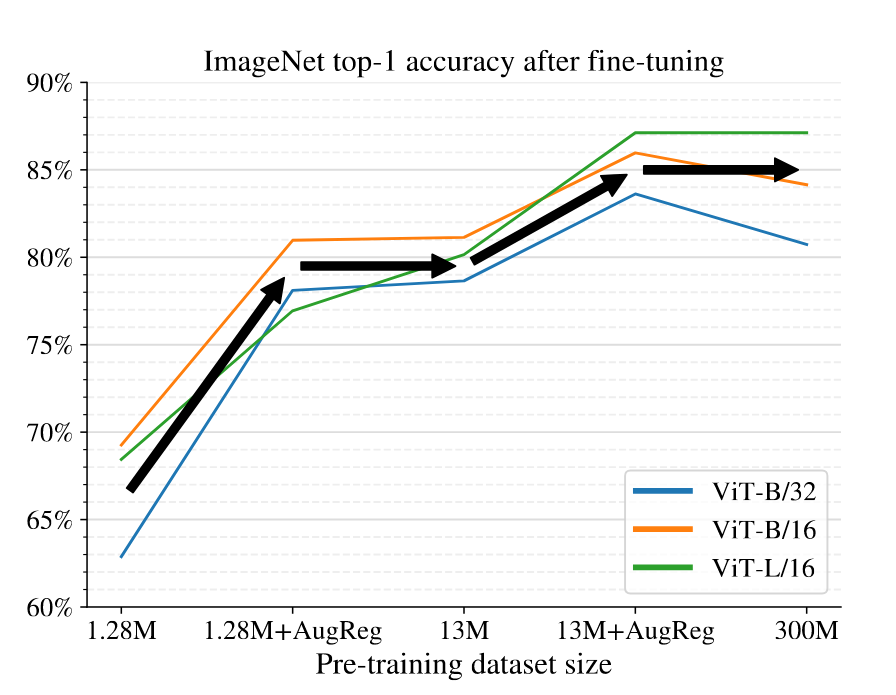
\includegraphics[width=0.95\linewidth]{augreg.png}
      \scriptsize \\
      Figure. Adding the right amount of regularization and image augmentation can lead to similar gains as increasing the dataset size by an order of magnitude.~\parencite{steinerHowTrainYour2022}
    \end{minipage}
    \bottomleftrefs
  \end{frame}
  \end{refsection}
  
  %--- Data Augmentation: How? ---
  \begin{refsection}
  \begin{frame}{How Do We Augment Data?}
    \textbf{Classic Methods:}
      \begin{itemize}
        \item Flip, rotate, crop, change colors, etc.
      \end{itemize}
      \textbf{Modern Methods:}
      \begin{itemize}
        \item Mix two images together (Mixup)~\parencite{zhangMixupEMPIRICALRISK2018}.
        \item Cut and paste parts of images (CutMix)~\parencite{yunCutMixRegularizationStrategy2019}.
      \end{itemize}
    \begin{minipage}{0.58\linewidth}
      \begin{figure}
        \centering
        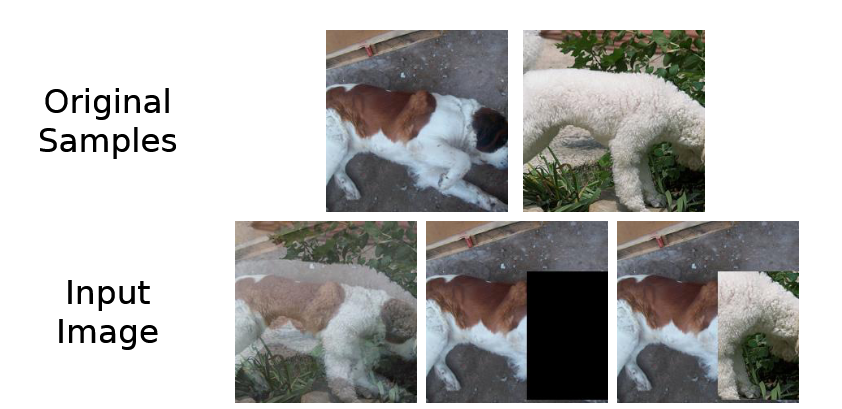
\includegraphics[width=0.6\linewidth]{aug_new_methods.png}
        \caption[]{\scriptsize Illustration of modern augmentation methods. From Left to Right: Mixup~\parencite{zhangMixupEMPIRICALRISK2018}, Cutout~\parencite{devriesImprovedRegularizationConvolutional2017}, and CutMix~\parencite{yunCutMixRegularizationStrategy2019}.}
      \end{figure}
    \end{minipage}
    \hfill
    \begin{minipage}{0.4\linewidth}
      \textbf{Soft Label Example (CutMix):}
      % \vspace{0.5em}
      \tiny
      \begin{equation*}
        \text{cutmix\_label} = \lambda \cdot \text{label}_A + (1 - \lambda) \cdot \text{label}_B
      \end{equation*}
      \vspace{-0.5em}
      \begin{equation*}
        \text{Example:} \quad \lambda = 0.5, \quad \text{label}_A = [1, 0], \quad \text{label}_B = [0, 1]
      \end{equation*}
      \vspace{-0.5em}
      \begin{equation*}
        \text{cutmix\_label} = 0.5 \times [1, 0] + 0.5 \times [0, 1] = [0.5, 0.5]
      \end{equation*}
     
  
    \end{minipage}
    \bottomleftrefs
  \end{frame}
  \end{refsection}
  
  
  
  %--- Generative Models for Data Augmentation ---
  \begin{refsection}
  \begin{frame}{Using Gen AI to Make New Images}
    \begin{itemize}
      \item Generative models can create new, realistic images.
      \item We can use them to make more training data.
      \item Example: Give a “before” image and a description, get a new “after” image.
    \end{itemize}
    \centering
    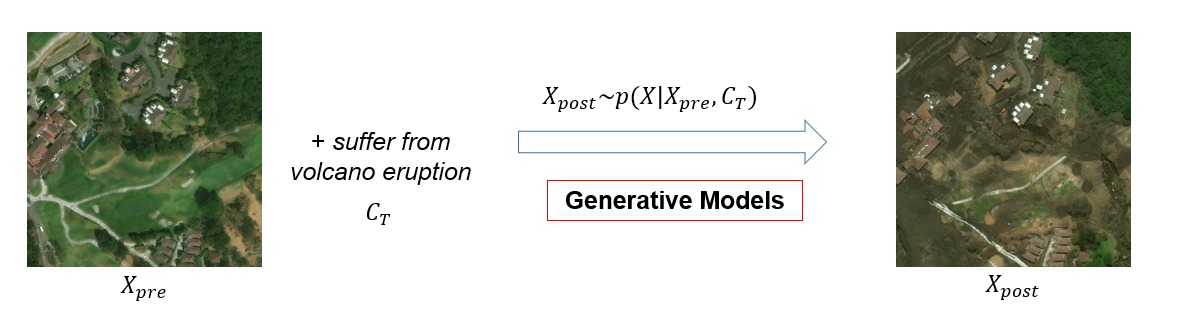
\includegraphics[width=1.0\linewidth]{diffusion_editing.png}
  \end{frame}
  \end{refsection}
  
  %--- Real-World Example: Disaster Images (xBD) ---
  \begin{frame}
    \centering
    \vspace{2.5cm}
    {\LARGE \textbf{Real-World Example: Disaster Images (xBD)}}
  \end{frame}
  
  \begin{refsection}
    \begin{frame}{xBD: A Large-Scale Disaster Damage Dataset}
      \begin{minipage}{0.42\linewidth}
        \centering
        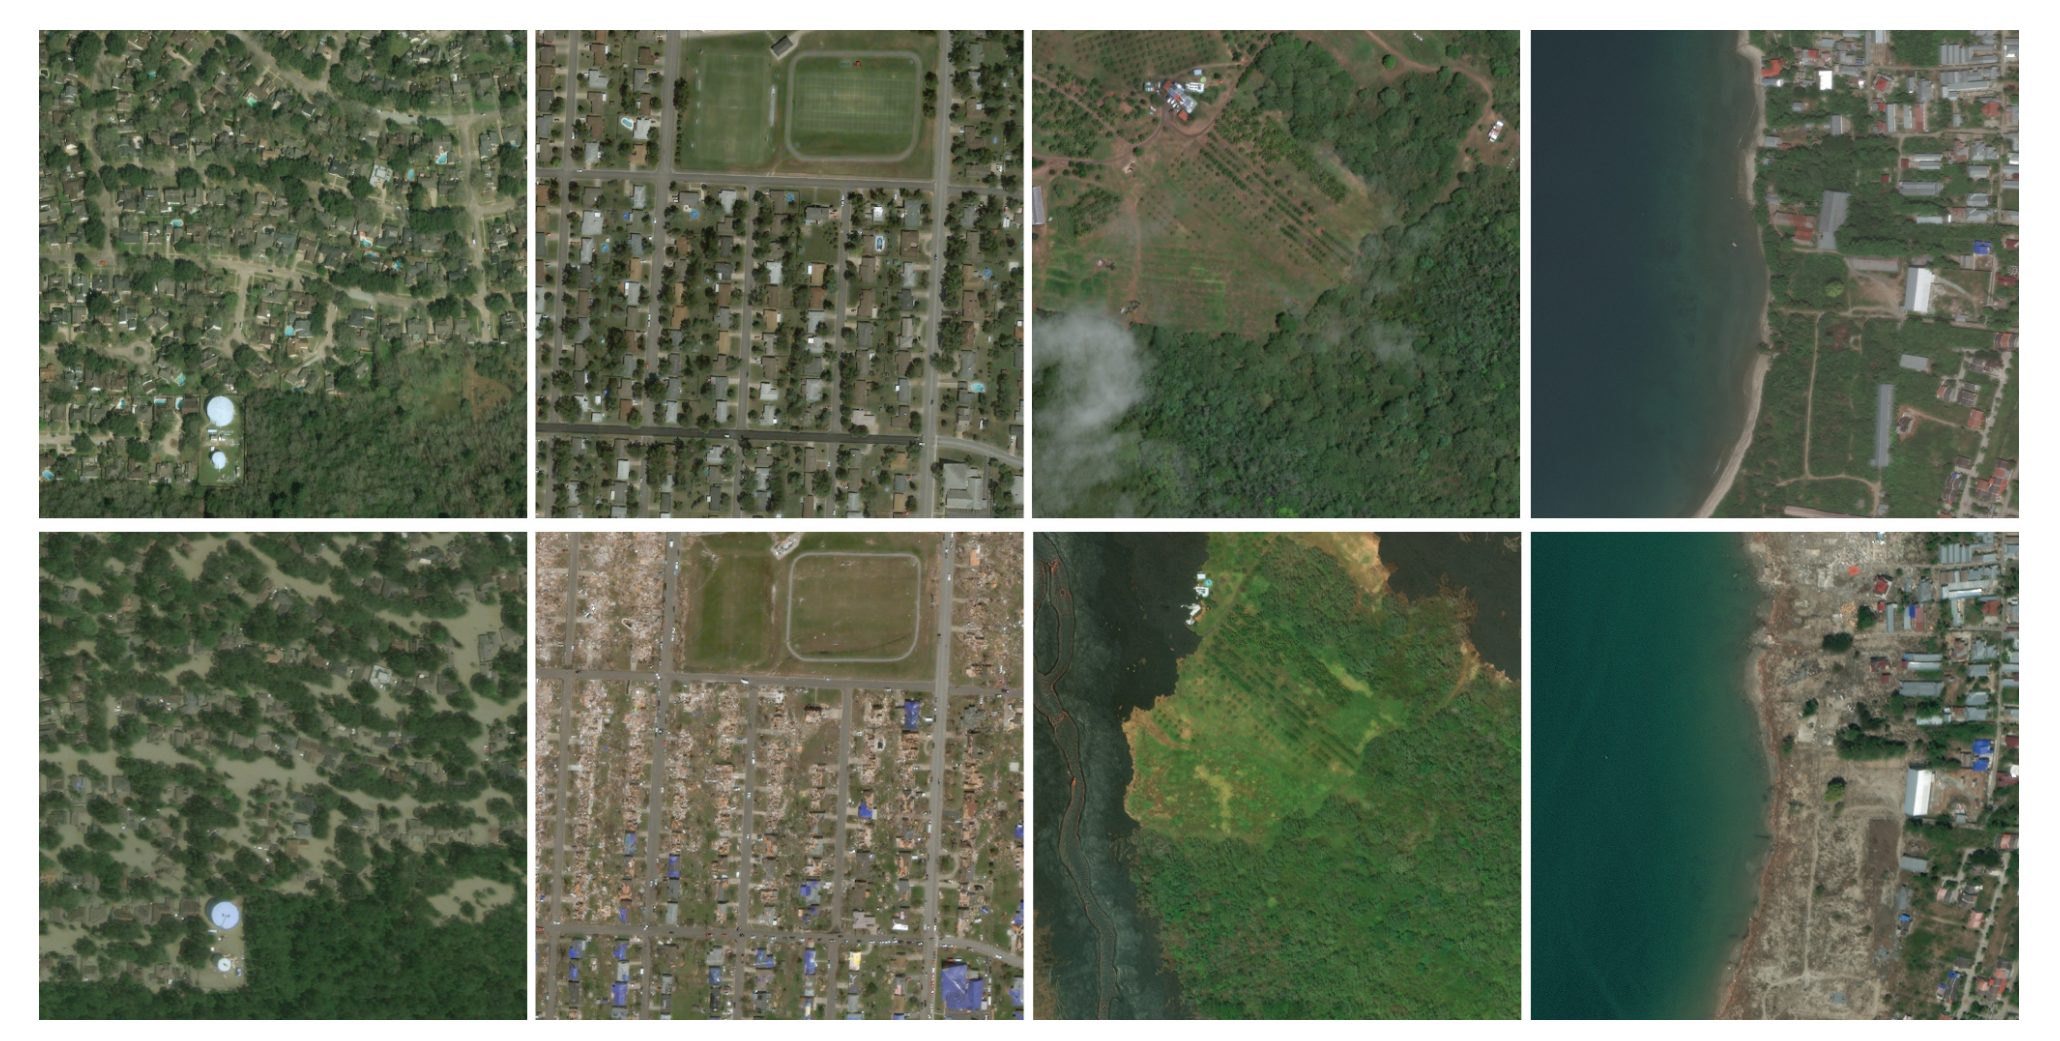
\includegraphics[width=1.0\linewidth]{xbd_samples.png}
        \vspace{0.5em}
        \scriptsize
        \textbf{xBD}~\parencite{guptaCreatingXBDDataset2019} is a bi-temporal remote sensing dataset covering 19 distinct disaster events. Pre-disaster imagery (top) and post-disaster imagery (bottom). From left to right: Hurricane Harvey; Joplin tornado; Lower Puna volcanic eruption; Sunda Strait tsunami.
      \end{minipage}%
      \hfill
      \begin{minipage}{0.55\linewidth}
        \tiny
        \centering
        \textbf{Table. 19 Disaster events in xBD.}
        \begin{tabular}{lll}
          \hline
          \textbf{Disaster Type} & \textbf{Disaster Event} & \textbf{Event Date} \\
          \hline
          Earthquake & Mexico City earthquake & Sep 19, 2017 \\
          Wildfire & Portugal wildfires & Jun 17--24, 2017 \\
          Wildfire & Santa Rosa wildfires & Oct 8--31, 2017 \\
          Wildfire & Carr wildfire & Jul 23--Aug 30, 2018 \\
          Wildfire & Woolsey fire & Nov 9--28, 2018 \\
          Wildfire & Piner fire & Nov 25--Dec 2, 2018 \\
          Volcano & Lower Puna volcanic eruption & May 23--Aug 14, 2018 \\
          Volcano & Guatemala Fuego volcanic eruption & Jun 3, 2018 \\
          Storm & Tuscaloosa, AL tornado & Apr 27, 2011 \\
          Storm & Joplin, MO tornado & May 22, 2011 \\
          Storm & Moore, OK tornado & May 20, 2013 \\
          Storm & Hurricane Matthew & Sep 28--Oct 10, 2016 \\
          Storm & Hurricane Florence & Sep 10--19, 2018 \\
          Flooding & Monsoon in Nepal, India, and Bangladesh & Aug 2017 \\
          Flooding & Hurricane Harvey & Aug 17--Sep 7, 2017 \\
          Flooding & Hurricane Michael & Oct 7--16, 2018 \\
          Flooding & Midwest US floods & Jan 3--May 31, 2019 \\
          Tsunami & Indonesia tsunami & Sep 18, 2018 \\
          Tsunami & Sunda Strait tsunami & Dec 22, 2018 \\
          \hline
        \end{tabular}
        \vspace{0.5em}
  
      \end{minipage}
      \bottomleftrefs
    \end{frame}
  \end{refsection}
  
  %--- Project Section ---
  \begin{frame}
    \centering
    \vspace{2.5cm}
    {\LARGE \textbf{Project: Can AI-Generated Images Help?}}
  \end{frame}
  
  %--- Project: What Will You Do? ---
  \begin{refsection}
  \begin{frame}{Project: What Will You Do?}
    \begin{itemize}
      \item Test if adding AI-generated images helps the model learn.
      \item Try three ways:
        \begin{itemize}
          \item Only real images
          \item Only generated images
          \item Both real and generated images
        \end{itemize}
      \item See which way gives the best results!
    \end{itemize}
  \end{frame}
  \end{refsection}
  
  %--- Project: Dataset & Image Generation ---
  \begin{refsection}
  \begin{frame}{Project: Dataset Details \& How to Generate Images}
    \begin{itemize}
      \item Use 100 real images per disaster type (6 types, 600 images total).
      \item For each type, generate 100–400 new images using AI.
      \item Try different mixes: 1:1, 1:2, 1:3, 1:4 (real:generated).
      \item Use commercial AI models (e.g., GPT-Image-1~\parencite{gptimage1}, Gemini 2.5 Pro~\parencite{geminiteamgoogleGemini25Pushing}, SeedEdit 3.0~\parencite{wang2025seedit}) to generate images.
      \item Input: a “before” image and a short description (e.g., “make it suffer from flooding”).
      \item Output: a new, realistic “after” image.
    \end{itemize}
    \bottomleftrefs
  \end{frame}
  \end{refsection}
  
  %--- Project: Models & Evaluation ---
  \begin{refsection}
  \begin{frame}{Which Models to Use \& How to Measure Success}
    \begin{itemize}
      \item \textbf{Try these models:}
        \begin{itemize}
          \item CLIPSeg~\parencite{luddeckeImageSegmentationUsing2022}
          \item MaskCLIP~\parencite{zhouExtractFreeDense2022}
          \item ClearCLIP~\parencite{lanClearCLIPDecomposingCLIP2024}
        \end{itemize}
      \item \textbf{How to measure success:}
      \begin{itemize}
        \item Use standard metrics for segmentation:
          \begin{itemize}
            \item \textbf{IoU (Intersection over Union):} Measures overlap between predicted and true regions.
            \item \textbf{F1 Score:} Harmonic mean of precision and recall for segmentation.
            \item \textbf{Pixel Accuracy:} Percentage of correctly classified pixels.
          \end{itemize}
        \item Compare results for each data mix (real, generated, both).
        \item Visualize and analyze which combination works best.
      \end{itemize}
    \end{itemize}
    \bottomleftrefs
  \end{frame}
  \end{refsection}
